

\tikzset{every picture/.style={line width=0.75pt}} %set default line width to 0.75pt        

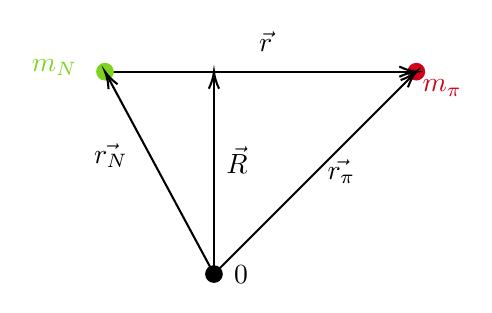
\begin{tikzpicture}[x=0.75pt,y=0.75pt,yscale=-0.75,xscale=0.75]
	%uncomment if require: \path (0,300); %set diagram left start at 0, and has height of 300
	
	%Flowchart: Connector [id:dp9827455772611288] 
	\draw  [color={rgb, 255:red, 208; green, 2; blue, 27 }  ,draw opacity=1 ][fill={rgb, 255:red, 208; green, 2; blue, 27 }  ,fill opacity=1 ] (315,90) .. controls (315,87.24) and (317.24,85) .. (320,85) .. controls (322.76,85) and (325,87.24) .. (325,90) .. controls (325,92.76) and (322.76,95) .. (320,95) .. controls (317.24,95) and (315,92.76) .. (315,90) -- cycle ;
	%Straight Lines [id:da5093684133345362] 
	\draw    (125,90) -- (318,90) ;
	\draw [shift={(320,90)}, rotate = 180] [color={rgb, 255:red, 0; green, 0; blue, 0 }  ][line width=0.75]    (10.93,-3.29) .. controls (6.95,-1.4) and (3.31,-0.3) .. (0,0) .. controls (3.31,0.3) and (6.95,1.4) .. (10.93,3.29)   ;
	%Straight Lines [id:da04984112064582158] 
	\draw    (190,220) -- (190,92) ;
	\draw [shift={(190,90)}, rotate = 90] [color={rgb, 255:red, 0; green, 0; blue, 0 }  ][line width=0.75]    (10.93,-3.29) .. controls (6.95,-1.4) and (3.31,-0.3) .. (0,0) .. controls (3.31,0.3) and (6.95,1.4) .. (10.93,3.29)   ;
	%Straight Lines [id:da13661676787341415] 
	\draw    (190,220) -- (318.59,91.41) ;
	\draw [shift={(320,90)}, rotate = 135] [color={rgb, 255:red, 0; green, 0; blue, 0 }  ][line width=0.75]    (10.93,-3.29) .. controls (6.95,-1.4) and (3.31,-0.3) .. (0,0) .. controls (3.31,0.3) and (6.95,1.4) .. (10.93,3.29)   ;
	%Flowchart: Connector [id:dp37210275318157304] 
	\draw  [color={rgb, 255:red, 126; green, 211; blue, 33 }  ,draw opacity=1 ][fill={rgb, 255:red, 126; green, 211; blue, 33 }  ,fill opacity=1 ] (115,90) .. controls (115,87.24) and (117.24,85) .. (120,85) .. controls (122.76,85) and (125,87.24) .. (125,90) .. controls (125,92.76) and (122.76,95) .. (120,95) .. controls (117.24,95) and (115,92.76) .. (115,90) -- cycle ;
	%Straight Lines [id:da8769015497622031] 
	\draw    (190,220) -- (120.95,91.76) ;
	\draw [shift={(120,90)}, rotate = 61.7] [color={rgb, 255:red, 0; green, 0; blue, 0 }  ][line width=0.75]    (10.93,-3.29) .. controls (6.95,-1.4) and (3.31,-0.3) .. (0,0) .. controls (3.31,0.3) and (6.95,1.4) .. (10.93,3.29)   ;
	%Flowchart: Connector [id:dp5562170943538245] 
	\draw  [color={rgb, 255:red, 0; green, 0; blue, 0 }  ,draw opacity=1 ][fill={rgb, 255:red, 0; green, 0; blue, 0 }  ,fill opacity=1 ] (185,220) .. controls (185,217.24) and (187.24,215) .. (190,215) .. controls (192.76,215) and (195,217.24) .. (195,220) .. controls (195,222.76) and (192.76,225) .. (190,225) .. controls (187.24,225) and (185,222.76) .. (185,220) -- cycle ;
	
	% Text Node
	\draw (71,80.4) node [anchor=north west][inner sep=0.75pt]  [color={rgb, 255:red, 126; green, 211; blue, 33 }  ,opacity=1 ]  {$m_{N}$};
	% Text Node
	\draw (322,93.4) node [anchor=north west][inner sep=0.75pt]  [color={rgb, 255:red, 208; green, 2; blue, 27 }  ,opacity=1 ]  {$m_{\pi }$};
	% Text Node
	\draw (196,136.4) node [anchor=north west][inner sep=0.75pt]    {$\vec{R}$};
	% Text Node
	\draw (261,144.4) node [anchor=north west][inner sep=0.75pt]    {$\vec{r_{\pi }}$};
	% Text Node
	\draw (111,134.4) node [anchor=north west][inner sep=0.75pt]    {$\vec{r_{N}}$};
	% Text Node
	\draw (217,62.4) node [anchor=north west][inner sep=0.75pt]    {$\vec{r}$};
	% Text Node
	\draw (201,212.4) node [anchor=north west][inner sep=0.75pt]    {$0$};
	
	
\end{tikzpicture}